\documentclass[a4paper, 11pt]{article}
%\usepackage[utf8]{inputenc}
\usepackage[T1]{fontenc}
\usepackage{tgpagella}
\usepackage[english]{babel}
\usepackage{amsmath,amsfonts,amssymb,amsthm}
%\usepackage{mathtools}
\usepackage{graphicx}
\usepackage{xcolor}
\usepackage{setspace}
\usepackage{multirow}
\usepackage{comment}
\usepackage{adjustbox, lscape, pdflscape, rotating, subfigure}
\usepackage[paper=portrait,pagesize]{typearea}
% \usepackage[a4paper, total={6in, 8in}]{geometry}
\usepackage{tgpagella}
\usepackage[top=2.5cm, left=2.0cm, right=2.0cm, bottom=3.0cm]{geometry}
\usepackage{amssymb,amsmath,amsfonts,booktabs,eurosym,geometry,ulem,graphicx,caption,color,setspace,sectsty,comment,footmisc,caption,natbib,pdflscape,subfigure,array,bbm}


\usepackage[colorlinks=true,linkcolor=red,linkcolor={black},citecolor={blue}]{hyperref}
\normalem



\newcommand\tzuhao[1]{\textcolor{blue}{{Tzu-Hao: }{#1}}}
\newcommand\tinghsiang[1]{\textcolor{olive}{{Ting-Hsiang: }{#1}}}
\newcommand\jingyang[1]{\textcolor{purple}{{Jingyang: }{#1}}}
\newcommand\wenjie[1]{\textcolor{red}{{Wenjie: }{#1}}}

\title{%
\begin{center}
    
\includegraphics[scale=0.1]{images/ETH.png}
\end{center}
\vspace{4em}
    % \textsc{A Geospatial Analysis of Crime in Chicago}
    \textsc{The Impact of Transit System on Local Crime: Evidence from Chicago's Transit System}
}

\author{Tzu-Hao Yan \and Lawrence Tseng \and Jingyang Wang \and Wenjie Tu}

\date{Fall Semester 2021}

\setlength{\parindent}{0pt}
\setlength{\parskip}{1em}
% \doublespacing
\onehalfspacing

\begin{document}

\clearpage
\maketitle
\thispagestyle{empty}


\begin{abstract}
\noindent This paper examines the impact of station on local crime events. Using spatial data from Chicago Data Portal, we propose an OLS model to capture the impact of transit system on local crime. We construct treatment and control zones in a way that there is little difference among these zones in terms of socioeconomic characteristics. The main result suggests a positive impact of transit system on local crime and we claim our finding causal. We discuss the potential causal channel that could explain our finding. We argue that stations provide a number of unique settings across which crime can occur: hard to monitor, easy to escape, more potential victims and offenders.

\vspace{4mm}

\noindent\textbf{Keywords:} Transit System; Crime; Geospatial Analysis; Causal Inference

\end{abstract}




\newpage
\setcounter{page}{1}
\doublespacing


%---------------------------------------------------------------------------------------
\section{Introduction} \label{sec:introduction}

Geographical approach and an interest for crime research have significantly increased over the last few decades due to the fact that crime cannot be separate from the offender’s natural habitat (\cite{herchenrader2015}). A link between human geography and criminology has been established as a result of the development of strong parallel that has existed in science for decades, similar to how criminology was predominantly put in the focus of sociology due to the series of paradigm shifts (\cite{butorac2017}). 

% Crimes and fear of crime affect many aspects of everyday life in our cities. Many studies have sought to document and analyze the different features which affect the occurrence of crimes. Especially for transit agencies, who usually instigated crime prevention strategies since crime affects people’s decisions to use public transportation, from which acts and perceptions of violence cause loss of ridership and revenue. 

% On the other hand, many studies had proven that the increase in passenger flow in certain areas may result in a higher crime rate, while establishing well-designed public transportation systems to increase passenger flow had also been proven to have a positive effect on economic development. Therefore, it is crucial to study the relationship between the crime rate and the public transportation system. 

The possible relationship between public transit and crime has been a controversial issue for many years. Some think that transit provides a number of unique settings (e.g., overcrowding) across which crime can occur, whereas others argue that it is the transit station's surrounding socioeconomic characteristics (e.g., population density and ethnicity) that affect the amount and the type of crime in the area.

% In this study, we analyze the relationship between the existence of subway stations and crime with a focus on Chicago. In the next section, a literature review of the related topics is provided. In section 3, the applied data structure and the model with a practical case are proposed. Followed by the result, discussion and a conclusion.

This paper examines the relationship between the existence of subway stations and crime with a focus on Chicago. The remainder of the article is structured as follows. Section \ref{sec:literature-review} presents the previous research on this topic. Section \ref{sec:methodology} describes the data and the empirical strategy. Section \ref{sec:results} demonstrates regression results. Section \ref{sec:discussion} illustrates the potential causal channel. Section \ref{sec:conclusion} concludes.

%----------------------------------------------------------------------------------------
\section{Literature Review \label{sec:literature-review}}

There has been an increasing concern over local crime in U.S. especially in Chicago. \cite{fear} argued that personal security can have a significant influence on travel patterns. \cite{pattern} found that public concerns over safety may be one of the most important reasons why many choose not to use transit.
 
 
% In terms of the cause of crime, there have been various perspectives to look at including socioeconomic characteristics of urban residents. Recent ecological approaches tend to analyze the micro-environment of crime, the social and spatial characteristics of the behavior settings in which crime takes place. From the studies with regard to the issue, we can know the following facts: explicit in criminological theories is the importance of place as a setting of crime. 

In terms of the cause of crime, there have been various perspectives to look at including socioeconomic characteristics of urban residents. Recent ecological approaches tend to analyze the micro-environment of crime, the social and spatial characteristics of the behavior settings in which crime takes place. \cite{felson1994crime} found that the particular sociophysical characteristics of a place (such as the number of people present, the level of surveillability, its physical layout, and environmental attributes) can have positive or negative effects on crime. \cite{degeneste1994policing} argued that most crime incidents occur in stations rather than on trains, and \cite{bus} also argued that crime is more likely to occur at bus stops rather than on buses, since the presence of the train crew or bus driver probably discourages potential offenders. Theorists also see transit stations as prime settings where crime against persons can be facilitated.

% The particular sociophysical characteristics of a place (such as the number of people present, the level of surveillability, its physical layout, and environmental attributes) can have positive or negative effects on crime.(\cite{felson1994crime}) Most crime incidents occur in stations rather than on trains (\cite{degeneste1994policing}) and at bus stops rather than on buses (\cite{bus}) since the presence of the train crew or bus driver probably discourages potential offenders. Theorists also see transit stations as prime settings where crime against persons can be facilitated.

With regard to station design, underpass stations tend to have higher crime rates than overpass stations, presumably because of less visibility. \cite{environment} claimed that a number of hiding places (under stairways, behind pillars) in the dark underpass stations.Unlike many rail systems that are well integrated in their surroundings, the location of many Green Line platforms in the midst of a freeway negates the potential for natural surveillance from neighborhood.

As some studies have shown, different types of crime take place under different conditions. Crime at the platforms against people was strongly related to ridership—the busiest stations tended to concentrate the most serious crime. Less serious crime tended to be higher in stations located in dense neighborhoods with higher percentages of population with less than high school education. 

However, in spite of the reasoning of how transit stations impact on crime above, whether railway stations will inevitably result in more crime is still in debate. \cite{mass} found crime to be increased during the public transit systems’ (including railway and bus) strike in Los Angeles, CA. \cite{doi:10.1111/j.1467-9906.2011.00564.x} used the DiD method and a quasi-experimental design to study crime and the light rail transit system in the city of Charlotte and found that crime did not increase because of the construction or implementation of the light rail.

% In the following sections, we will set up our model to explore the relationship of existence of subway stations and crime with a focus on Chicago, which has been under high crime rates for long. 

In the following sections, we examine the relationship between transit system and crime in the city of Chicago to better understand such an issue.


%------------------------------------------------------------------------------------------
\section{Methodology} \label{sec:methodology}

\subsection{Data Source}

The datasets that we use in this project were obtained from the Chicago Data Portal. This website is operated by the City of Chicago to provide access to government data, which is collected, processed, and maintained by different agencies of the city government. The datasets used for this analysis include reported crime data, public transit information, and community characteristics, which are provided by Chicago Police Department, Chicago Transit Authority, and Chicago Department of Public Health, respectively. Descriptions of each dataset as well as the application in this project are demonstrated in the following paragraphs. 

\textbf{Crime data} 

The Chicago crime data used in this work details every crime event that occurred in the city between 2010 and 2019. This 10-year data is extracted from the original dataset with the crime data from 2001 to present in order to reduce the impacts from the financial crisis in 2008 and the COVID-19 pandemic. The extracted dataset contains 2,974,162 reported crime events, and each crime data records the information such as date and time of occurrence, type of crimes, location, and coordinates. Table \ref{tab:crime_data} contains a small subset of this data for reference. 

\vspace{0.5cm}
\begin{table}[!h] \centering
\caption{A small subset of the crime data used in this analysis.}
\label{tab:crime_data}
\begin{tabular}{ l l l c c c}
 \hline\hline
 Date and Time & Crime Type & Location & Community & Longitude & Latitude\\ 
 \hline
 9/5/2015 13:30 & BATTERY & RESIDENCE & 61 & -87.66 & 41.81 \\  
 9/4/2015 11:30 & THEFT & CTA BUS & 25 & -87.76 & 41.89 \\
 9/5/2015 12:45 & NARCOTICS & SIDEWALK & 21 & -87.72 & 41.94 \\
 9/5/2015 13:00 & ASSAULT & APARTMENT & 25 & -87.76 & 41.88 \\
 9/5/2015 10:55 & BURGLARY & RESIDENCE & 71 & -87.66 & 41.74 \\
 \hline\hline
\end{tabular}
\end{table}

\textbf{Public transit information}

The public transit information is provided by the Chicago Transit Authority (CTA), which operates the mass transit in Chicago, trains of Chicago ‘L’ and CTA bus service. The list of transit datasets include bus routes/subway lines, location of each bus stop/subway station, and average daily ridership for these two transit systems. In this project, we use the location of subway stations of different lines to analyze their impacts on local crime occurrence. 

\textbf{Chicago community area} 

The city of Chicago is divided into 77 community areas for statistical and planning purposes. The boundaries of communities were defined by the Social Science Research Committee at the University of Chicago and related municipal agencies in early 20th Century. Unlike census tracts that have been standardized and utilized to make census records across different counties in the United States, community areas are regarded more natural and manageable due to the consideration of physical barriers and the identity of local neighbourhoods. Additionally, community areas are more consistent, compared with wards (political subdivisions in Chicago), which change every 10 years. The current boundaries of community areas are mostly remained unchanged since they were introduced in the 1920s, local residents still refer to those communities by their original community names. 

\subsection{Spatial Data Processing}

The objective of this project is to evaluate the change of crime occurrence with respect to the existence of subway station. In order to reduce the effects of other socioeconomic characteristics that could significantly affect local crime rates, we selected three adjacent communities that share the relatively similar demographics, such as population density, income, and education level. The selected communities are Lake View, Lincoln Park, and Near North Side, and the rankings of these communities among all communities in Chicago with regard to the aforementioned characteristics as well as the overall socioeconomic score is demonstrated in Table \ref{tab:community_index}. We also adjust and simplify the boundary of combined communities to remove the area covered by park and river and to facilitate the analysis. The simplified study area is shown in Figure \ref{fig:station_samples} (a). 

\vspace{0.5cm}
\begin{table}[!h] \centering
\caption{Rankings of the selected communities in different socioeconomic characteristics.}
\label{tab:community_index}
\begin{tabular}{ l c c c c}
 \hline\hline
 Name & Density & Income Per Capita & Education Level & Overall Score \\ 
 \hline
 Lake View & 8 & 4 & 4 & 5\\  
 Lincoln Park & 2 & 2 & 2 & 2\\
 Near North Side & 1 & 1 & 1 & 1 \\
 \hline\hline
\end{tabular}
\end{table}

\begin{comment}
\begin{figure}[!tbp]
    \centering
    \begin{minipage}[b]{2cm}
        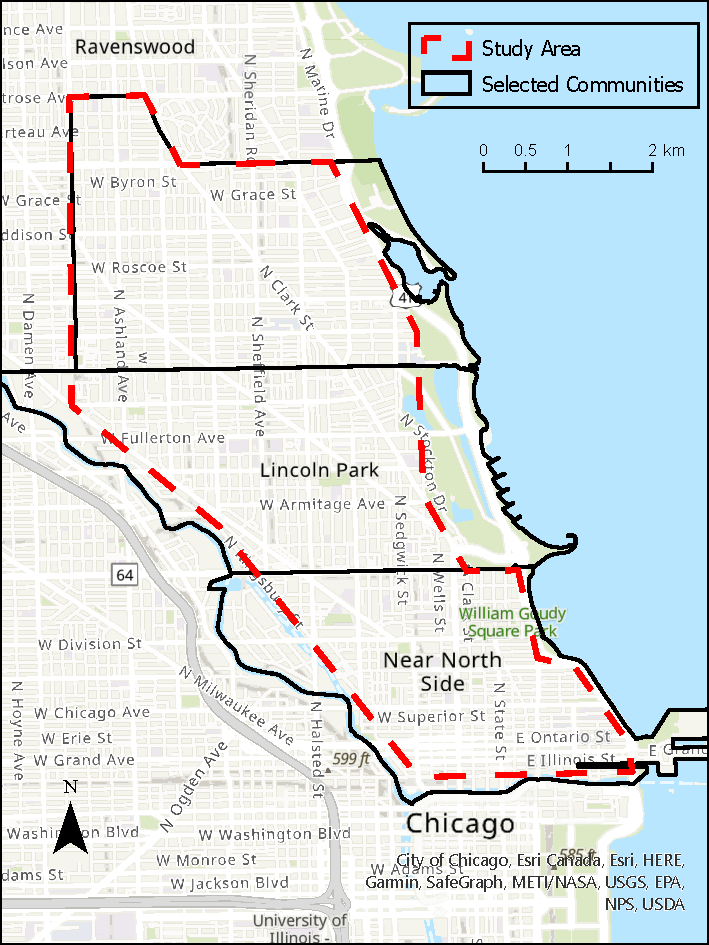
\includegraphics[width=8cm]{figures/study_area.pdf}
        \caption{Study Area}
        \label{fig:study_area}
    \end{minipage}
    \hfill
    \begin{minipage}[b]{-0.5cm}
        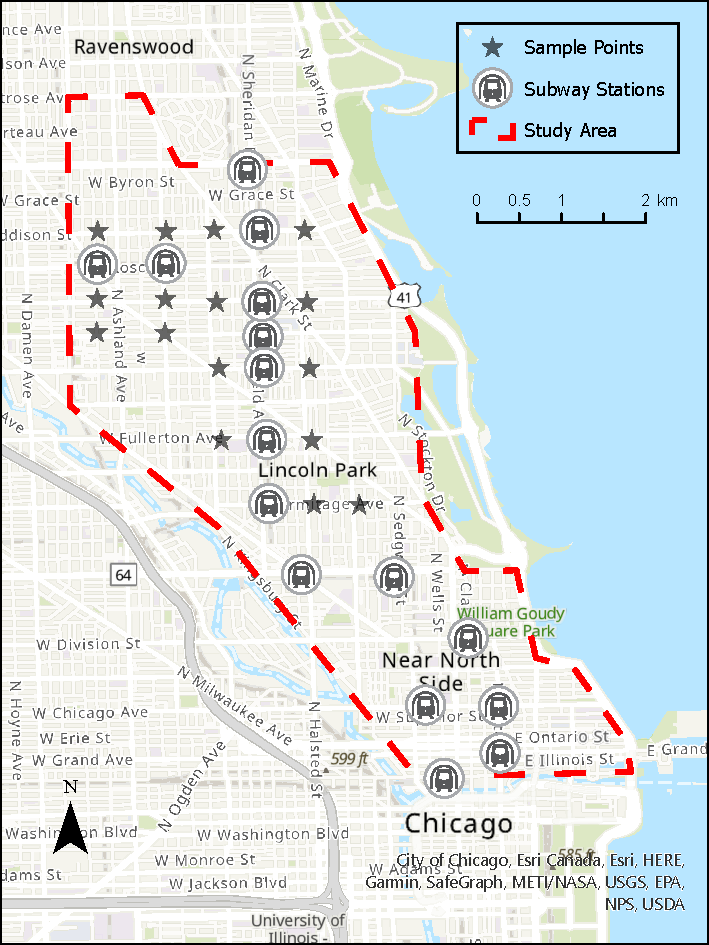
\includegraphics[width=8cm]{figures/stations_and_samples.pdf}
        \caption{Station and Sample Points}
        \label{station_samples}
    \end{minipage}

\end{figure}
\end{comment}

There are three subway lines and 16 stations provide service in the study area. We create 16 circular zones surrounding the subway stations with a radius of 200 meters to capture the amount of crime events near the subway stations in each year from 2010 to 2019. This is also applied to create another 16 zones without a station as the control units. The control units are randomly selected within the study area in a way that there is no overlap with the zones containing a station. The physical locations of station and control points are displayed in Figure \ref{fig:station_samples} (b).

\begin{figure}%
\hfill
\subfigure[Study Area]{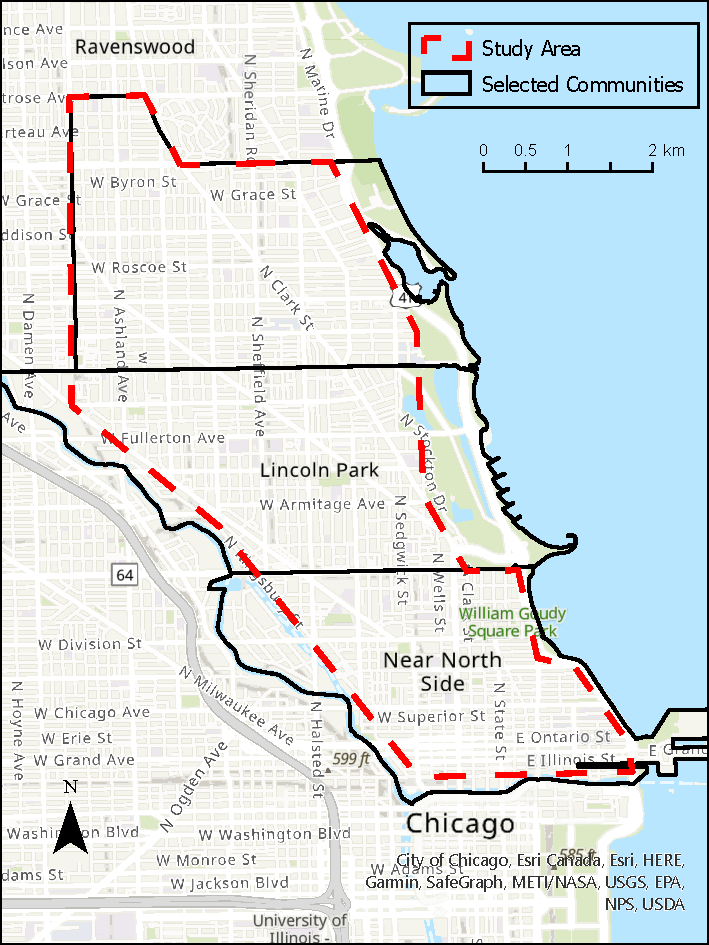
\includegraphics[scale=0.6]{figures/study_area.pdf}}
\hfill
\subfigure[Stations and Samples]{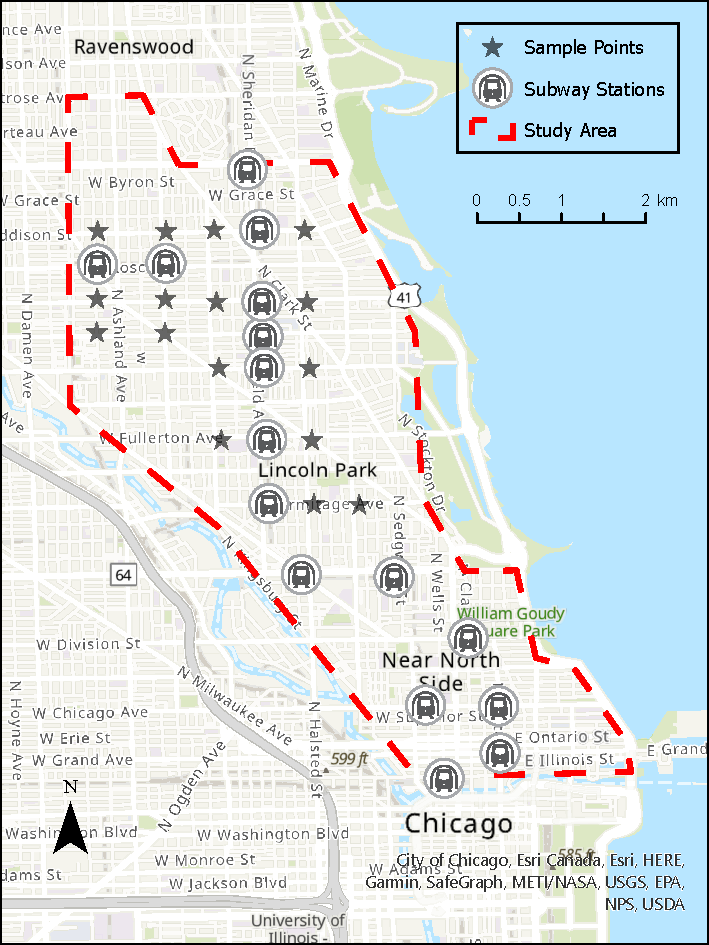
\includegraphics[scale=0.6]{figures/stations_and_samples.pdf}}
\hfill\hfill
\caption{The Area of Interest with Treatment and Control Units}
\label{fig:station_samples}
\end{figure}

\subsection{Theoretical Framework}

\textbf{Assumption 1 } \textit{Functional form:}

In this study, we want to estimate the effect of station on local crime. First, we assume that $\log Y_{it}$ takes in a linear form:

\[\log Y_{it}=\beta + \delta D_{it} + \epsilon_{it} \]

\begin{itemize}
    \item $Y_{it}$: the number of crime cases within area $i$ during year $t$.
    \item $D_{it}$: treatment indicator, which is equal to 1 if there is a transit within area $i$ in year $t$, and 0 otherwise.
    \item $\delta$: the average treatment effect averaged over all years.
    \item $\epsilon_{it}$: the error term.
\end{itemize}


In our model, the dependent variable is in log terms while the independent variable of interest is a dummy. In the log-dummy specification, the coefficient of interest has different interpretations in different contexts:

Case 1: if the estimated coefficient of interest is sufficiently close to 0, we can use the following approximation and interpret the estimate in percentage terms:

\begin{align*}
    \delta &= \mathbb{E}[\log Y_{it}\mid D_{it}=1] - \mathbb{E}[\log Y_{it}\mid D_{it}=0] \\
    &= \mathbb{E}[\log Y_1] - \mathbb{E}[\log Y_0] \\
    &= \mathbb{E}[\log Y_1 - \log Y_0] \\
    &= \mathbb{E}\left[\log\frac{Y_1}{Y_0}\right]
    \approx \mathbb{E}\left[\frac{Y_1 - Y_0}{Y_0} \right]
\end{align*}

Case 2: if the estimated coefficient of interest is away from zero, we should interpret the estimate as:

\begin{equation*}
     \frac{(Y_{it}\mid D_{it}=1) - (Y_{it}\mid D_{it}=0)}{Y_{it}\mid D_{it}=0}
    =\frac{e^{\alpha+\delta+\epsilon} - e^{\alpha+\epsilon}}{e^{\alpha+\epsilon}}=e^{\delta}-1
\end{equation*}

In order to estimate the average treatment for each year, we formulate another regression model. We also assume that $\log Y_i$ takes in the same linear form for each year:

\[\log Y_{i}=\alpha+\gamma_{t} D_{i}+\upsilon_{i} \]

\begin{itemize}
    \item $Y_{i}$: the number of crime cases within area $i$.
    \item $D_{i}$: treatment indicator, which is equal to 1 if there is a transit within area $i$, and 0 otherwise.
    \item $\gamma_t$: the average treatment effect for year $t$.
    \item $\upsilon_{i}$: the error term.
\end{itemize}

\textbf{Assumption 2 } \textit{Strict exogeneity:}

\[\epsilon_{it}\perp D_{it} \]

Assumption 2 means that the error term of any unit at any time period is independent of treatment assignment. A strict exogeneity assumption also implies conditional mean independence, i.e., $\mathbb{E}[\epsilon_{it}\mid D_{it}]=0$.

\textbf{Assumption 3 } \textit{Homoscedasticity:}

Homoscedasticity means that the variance of the error term is constant across different observations, i.e., $\mathrm{Var}(\epsilon_{it})=\sigma^2$.

\textbf{Assumption 4 } \textit{Weak serial dependence of the error terms:}

We assume that the covariance between any two error terms, $\epsilon_{i}$ and $\epsilon_{j}$, is zero, i.e., $\mathrm{Cov}(\epsilon_i,\epsilon_j)=0$.

\textbf{Assumption 5 } \textit{Normality:}

We assume that the error term $\epsilon_{it}$ is normally distributed. This assumption ensures that statistical tests are valid. Combined with previous assumptions, we can express this assumption as $\epsilon_{it}\mid D_{it}\sim\mathcal{N}(0, \sigma^2)$.


\subsection{Assumption Check}

We conduct regression diagnostics to evaluate the model assumptions. Figure \ref{fig:diagnostic} shows four diagnostic plots:

\begin{itemize}
    \item Linearity: the Residuals vs Fitted plot tests if residuals have non-linear patterns. We see from the top-left plot in Figure \ref{fig:diagnostic} that residuals are equally spread around a horizontal line without distinct patterns, which indicates that there exists no non-linear relationship in log-dummy specification.
    \item Normality: the Normal Q-Q plot tests if residuals are normally distributed. We see from the top-right plot in Figure \ref{fig:diagnostic} that residuals are lined well on the straight dashed line, which indicates that residuals are normally distributed with a mean of zero (i.e. $\mathbb{E}[\epsilon\mid D]=0$).
    \item Homoscedasticity: the Spread-Location plot tests of residuals are spread equally along the ranges of predictors. We can see from bottom-left plot in Figure \ref{fig:diagnostic} that there is a horizontal line with equally (randomly) spread points.
    \item Leverage Point: the Constant Leverage plot tests if there are any influential samples. We can see from bottom-left plot in Figure \ref{fig:diagnostic} that there are not many leverage points.
\end{itemize}

\begin{figure}
    \centering
    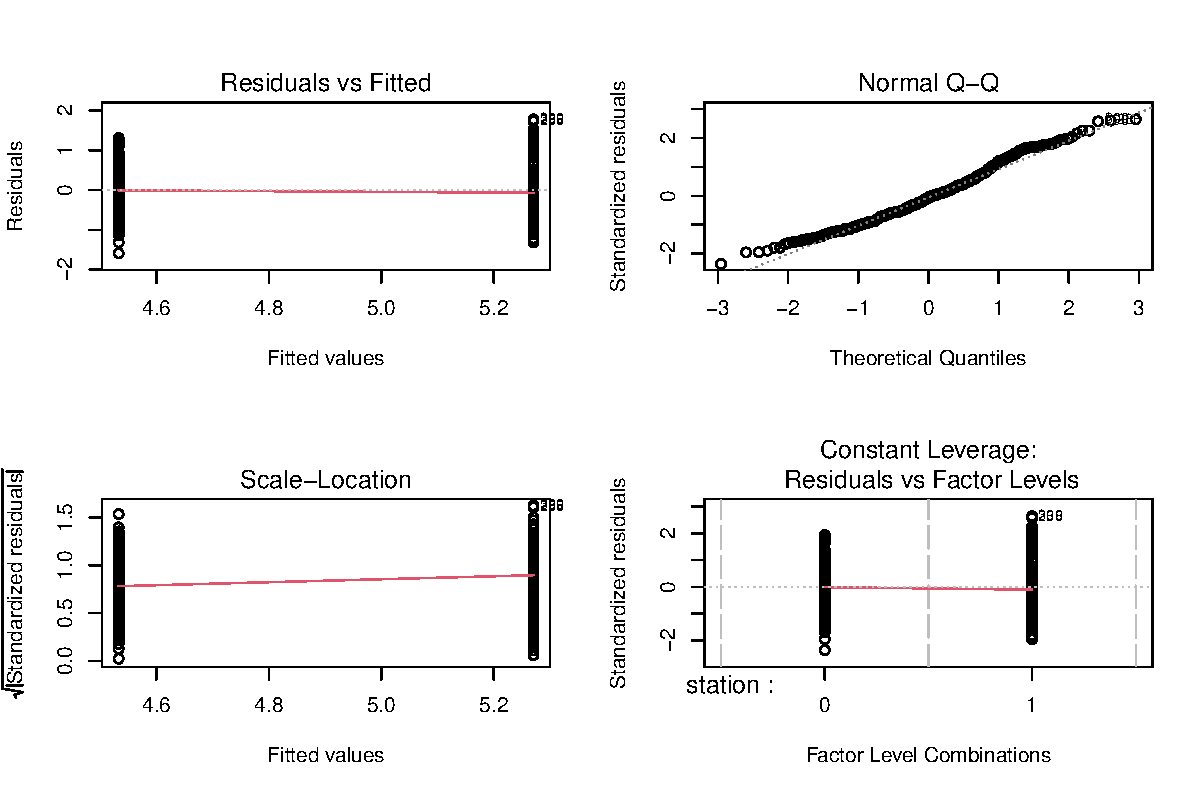
\includegraphics[scale=0.8]{figures/logplot.pdf}
    \caption{Diagnostic Plots}
    \label{fig:diagnostic}
\end{figure}


%----------------------------------------------------------------------------------------

\section{Results} \label{sec:results}

\begin{figure}%
\hfill
\subfigure[log(Crime) vs. Year]{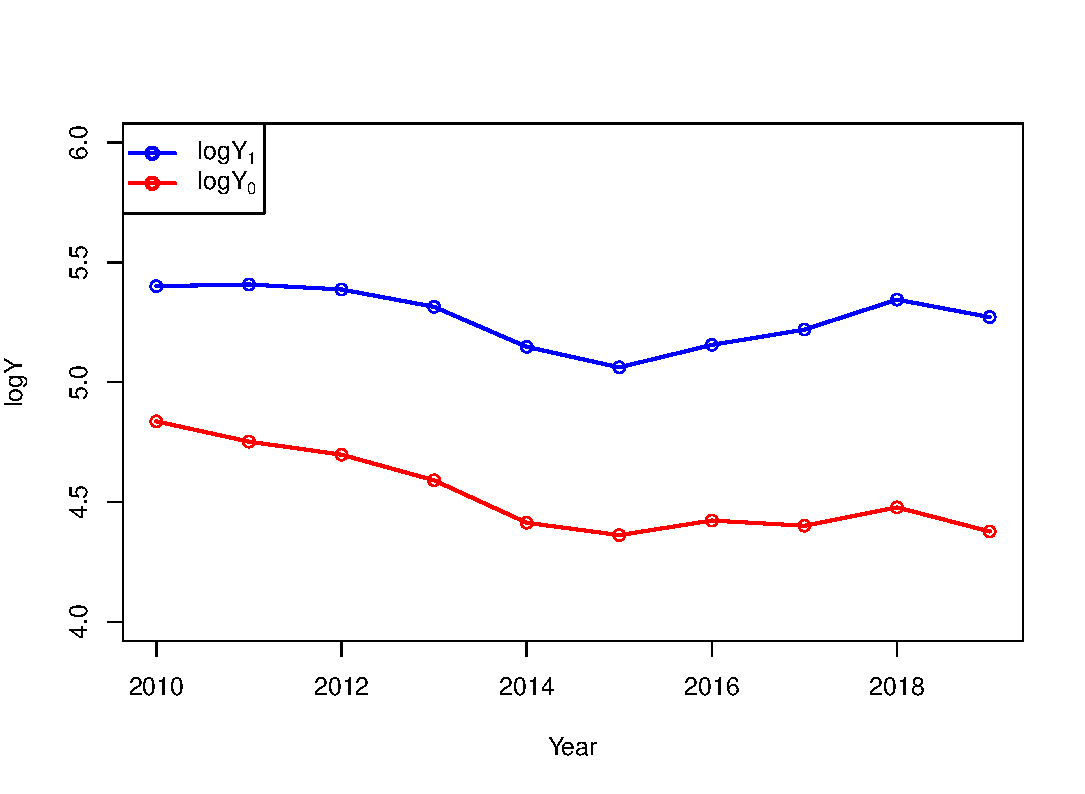
\includegraphics[scale=0.4]{figures/lncrime-year1.pdf}}
\hfill
\subfigure[Effect vs. Year]{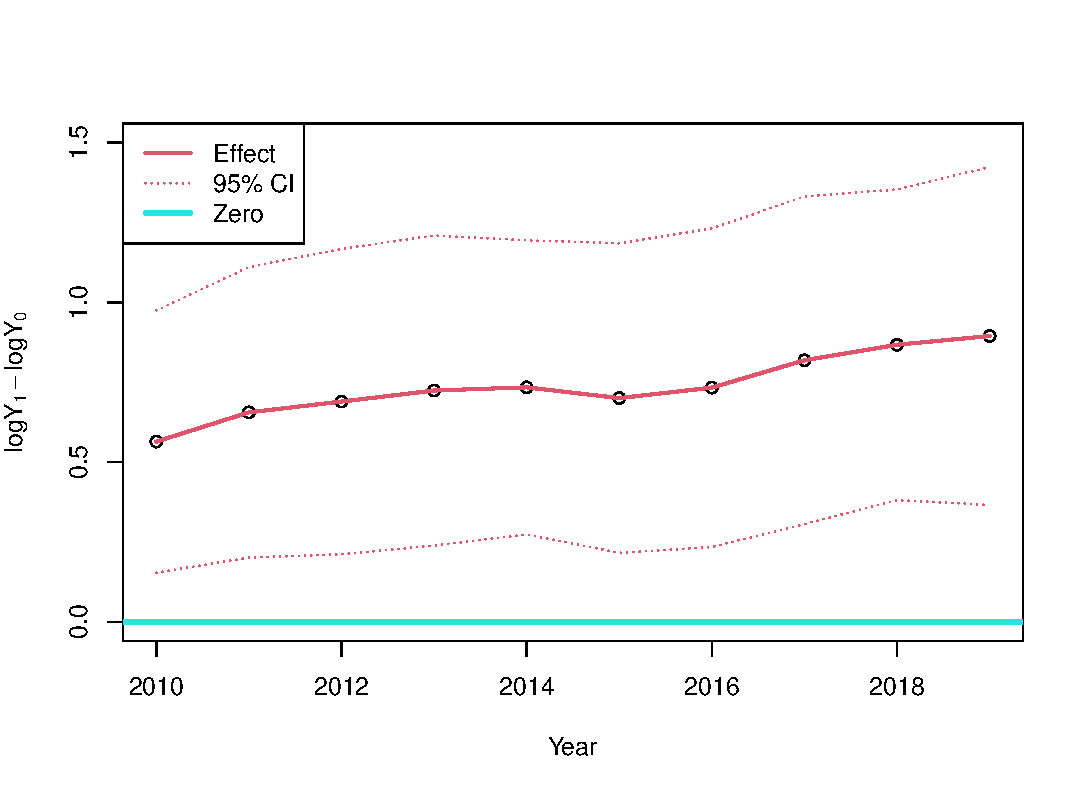
\includegraphics[scale=0.4]{figures/ate-year1.pdf}}
\hfill\hfill
\caption{Evolution of Crime over 10 Years}
\label{fig:results}
\end{figure}



% We would like to investigate how crime evolves over time in an area with and without station. 
We aggregate the data over each year and visualize it with crime in log terms as y axis and year as x axis. The unit level is a circular area with a radius of 200 meters. Figure \ref{fig:results} (a) demonstrates how crime in log terms evolves over the period from 2010 to 2019. We can clearly see that these two time series follow a similar trend. In other words, the gap between treatment group and control group is almost constant across different years and treatment and control groups demonstrate quasi-parallel trends in outcome. However, we can still detect that such a gap becomes slightly larger as time goes by. We will come back to this in the quantitative analysis.

% the treatment group is denoted by blue and control group is denoted by red. It is more intuitive and straightforward to see a clear pattern of the evolution of crime over the period from 2010 to 2019. It is worth noting that treatment and control groups demonstrate quasi-parallel trends in outcome (i.e., the gap between treatment group and control group is almost constant across different years). However, we can still notice that such a gap becomes larger as time goes by.

%------------------------------------------------------------------------------------

\begin{comment}
\begin{figure}
    \centering
    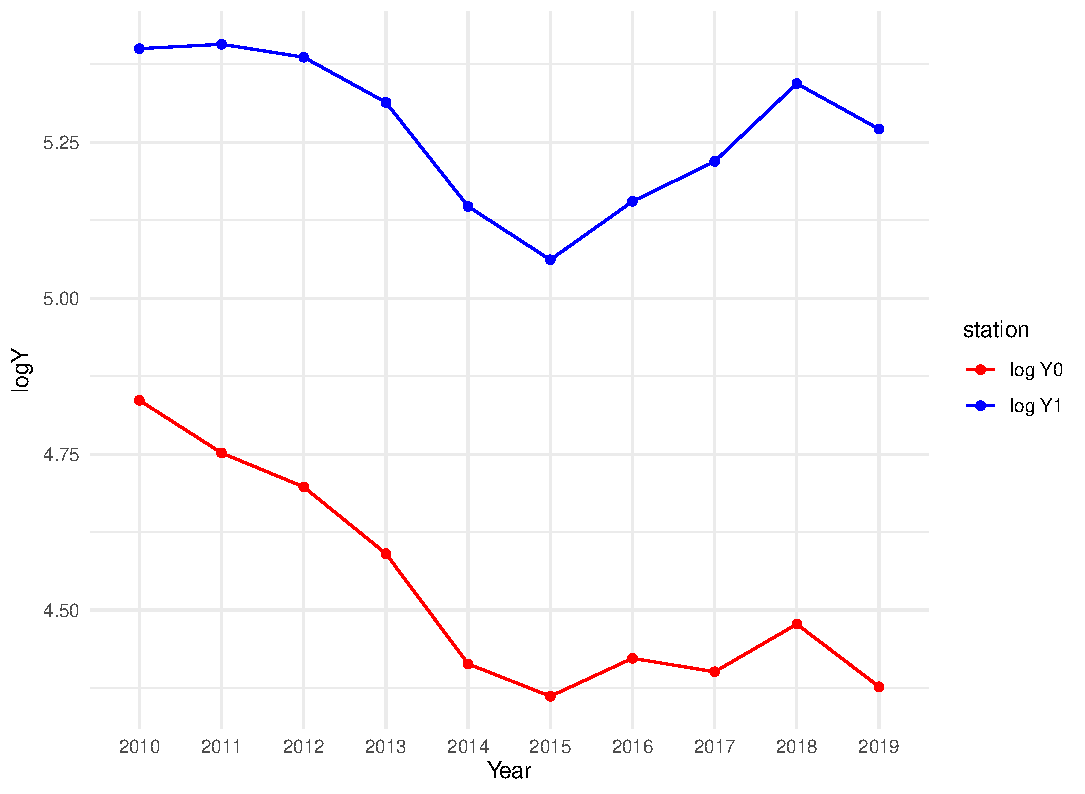
\includegraphics[scale=0.6]{figures/lncrime-year.pdf}
    \caption{log(Crime) vs. Year}
    \label{fig:lncrime-year}
\end{figure}

\begin{figure}
    \centering
    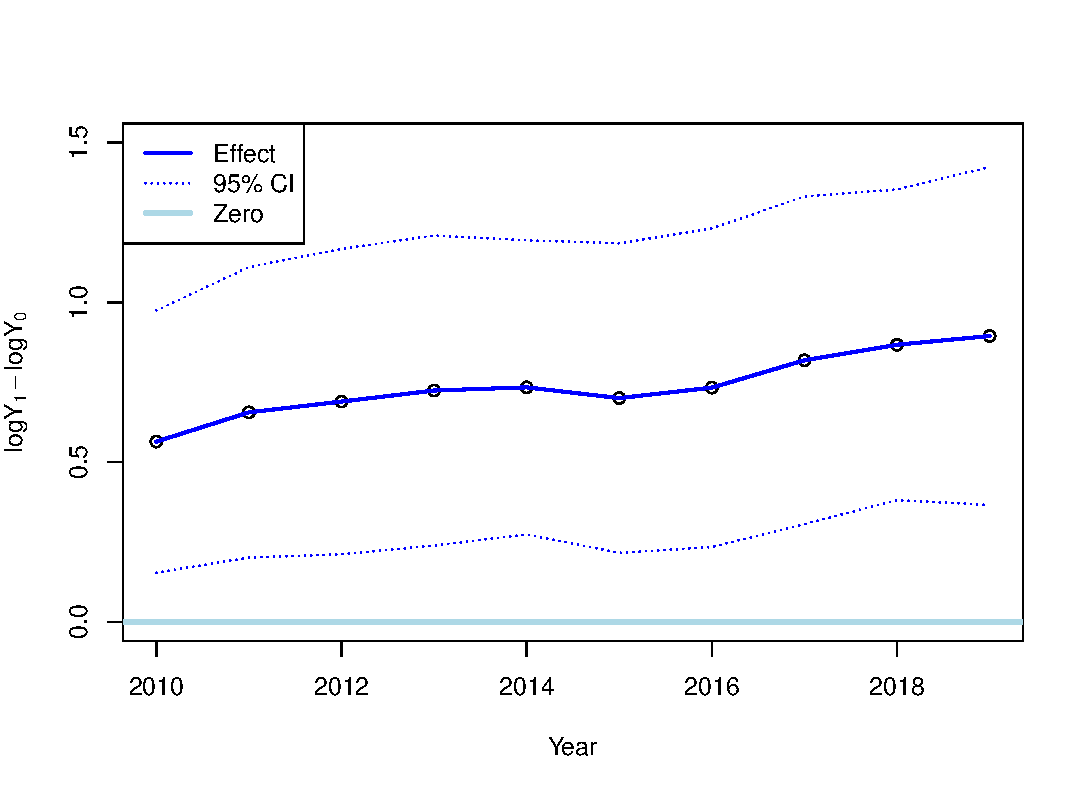
\includegraphics[scale=0.6]{figures/ate-year.pdf}
    \caption{Effect vs. Year}
    \label{fig:ate-year}
\end{figure}
\end{comment}

In order to gain a better idea of the effect size (i.e., the gap), we run 10 regressions to estimate the coefficient of interest for each year of the samples. As expected, Figure \ref{fig:results} (b) suggests an upward trend in the coefficient of interest. We draw 95\% confidence interval for each treatment coefficient. We can also clearly see that the coefficient of interest is significantly different from zero across all the years. We next turn to more technical and quantitative results. In Table \ref{tab:ate-year}, we can quantitatively see the exact impact size for each year. In log-dummy specification, the coefficient of interest is interpreted as the percentage changes. In 2010, there are 75.8\% ($e^{0.564}-1$) more crime cases on average in the areas with stations than in the areas without stations. Overall, we see that the treatment coefficient increases over time despite a slight drop in 2015.

We then run a full regression of crime in log terms on the treatment dummy variable over all the years (i.e. the average treatment effect averaged over 10 years). For comparison, we also run a regression of crime in level terms on the treatment dummy variable. In Figure \ref{fig:crime-qqplot}, we know that the normality assumption does not hold in level-dummy specification. We conduct a log transformation on the outcome variable to ensure that normality and mean-zero error assumptions hold. Figure \ref{fig:lncrime-qqplot} validates the log transformation. In Table \ref{tab: ate-all}, we see that the coefficient of interest in log-dummy specification is 0.738. The interpretation is that there are 109.2\% ($e^{0.738}-1$) more crime on average in the area with a station than in the area without a station. Such an effect is statistically different from zero at 0.01 significance level.

%---------------------------------------------------------------------------------------

\begin{comment}
\begin{table}[!htbp] \centering 
  \caption{} 
  \label{} 
\tiny 
\begin{tabular}{@{\extracolsep{5pt}}lcccccccccc} 
\\[-1.8ex]\hline 
\hline \\[-1.8ex] 
 & \multicolumn{10}{c}{\textit{Dependent variable:}} \\ 
\cline{2-11} 
\\[-1.8ex] & \multicolumn{10}{c}{lncrime} \\ 
 & 2010 & 2011 & 2012 & 2013 & 2014 & 2015 & 2016 & 2017 & 2018 & 2019 \\ 
\hline \\[-1.8ex] 
 station1 & 0.564$^{**}$ & 0.655$^{***}$ & 0.689$^{***}$ & 0.724$^{***}$ & 0.734$^{***}$ & 0.700$^{***}$ & 0.733$^{***}$ & 0.818$^{***}$ & 0.867$^{***}$ & 0.894$^{***}$ \\ 
  & (0.205) & (0.227) & (0.239) & (0.243) & (0.230) & (0.242) & (0.249) & (0.256) & (0.243) & (0.264) \\ 
  & & & & & & & & & & \\ 
 Constant & 4.836$^{***}$ & 4.752$^{***}$ & 4.697$^{***}$ & 4.590$^{***}$ & 4.414$^{***}$ & 4.362$^{***}$ & 4.423$^{***}$ & 4.401$^{***}$ & 4.477$^{***}$ & 4.377$^{***}$ \\ 
  & (0.145) & (0.161) & (0.169) & (0.171) & (0.163) & (0.171) & (0.176) & (0.181) & (0.172) & (0.187) \\ 
  & & & & & & & & & & \\ 
\hline \\[-1.8ex] 
Observations & 32 & 32 & 32 & 32 & 32 & 32 & 32 & 32 & 32 & 32 \\ 
R$^{2}$ & 0.201 & 0.217 & 0.217 & 0.229 & 0.253 & 0.218 & 0.224 & 0.254 & 0.298 & 0.276 \\ 
\hline 
\hline \\[-1.8ex] 
\textit{Note:}  & \multicolumn{10}{r}{$^{*}$p$<$0.1; $^{**}$p$<$0.05; $^{***}$p$<$0.01} \\ 
\end{tabular} 
\end{table} 
\end{comment}

%--------------------------------------------------------------------------------------


\begin{landscape}
\begin{table}[!htbp] \centering 
  \caption{Average Treatment Effect by Year} 
  \label{tab:ate-year} 
\begin{tabular}{@{\extracolsep{5pt}}lcccccccccc} 
\\[-1.8ex]\hline 
\hline \\[-1.8ex] 
 & \multicolumn{10}{c}{\textit{Dependent variable:}} \\ 
\cline{2-11} 
\\[-1.8ex] & \multicolumn{10}{c}{lncrime} \\ 
 & 2010 & 2011 & 2012 & 2013 & 2014 & 2015 & 2016 & 2017 & 2018 & 2019 \\ 
\hline \\[-1.8ex] 
 station1 & 0.564$^{**}$ & 0.655$^{***}$ & 0.689$^{***}$ & 0.724$^{***}$ & 0.734$^{***}$ & 0.700$^{***}$ & 0.733$^{***}$ & 0.818$^{***}$ & 0.867$^{***}$ & 0.894$^{***}$ \\ 
  & (0.205) & (0.227) & (0.239) & (0.243) & (0.230) & (0.242) & (0.249) & (0.256) & (0.243) & (0.264) \\ 
  & & & & & & & & & & \\ 
 Constant & 4.836$^{***}$ & 4.752$^{***}$ & 4.697$^{***}$ & 4.590$^{***}$ & 4.414$^{***}$ & 4.362$^{***}$ & 4.423$^{***}$ & 4.401$^{***}$ & 4.477$^{***}$ & 4.377$^{***}$ \\ 
  & (0.145) & (0.161) & (0.169) & (0.171) & (0.163) & (0.171) & (0.176) & (0.181) & (0.172) & (0.187) \\ 
  & & & & & & & & & & \\ 
\hline \\[-1.8ex] 
Observations & 32 & 32 & 32 & 32 & 32 & 32 & 32 & 32 & 32 & 32 \\ 
R$^{2}$ & 0.201 & 0.217 & 0.217 & 0.229 & 0.253 & 0.218 & 0.224 & 0.254 & 0.298 & 0.276 \\ 
\hline 
\hline \\[-1.8ex] 
\textit{Note:}  & \multicolumn{10}{r}{$^{*}$p$<$0.1; $^{**}$p$<$0.05; $^{***}$p$<$0.01} \\ 
\end{tabular} 
%\end{table} 

\vspace{4em}

%\begin{table}[!htbp] \centering 
  \caption{Average Treatment Effect Averaged over 10 Years} 
  \label{tab: ate-all} 
\begin{tabular}{@{\extracolsep{5pt}}lcc} 
\\[-1.8ex]\hline 
\hline \\[-1.8ex] 
 & \multicolumn{2}{c}{\textit{Dependent variable:}} \\ 
\cline{2-3} 
\\[-1.8ex] & crime & lncrime \\ 
\\[-1.8ex] & (1) & (2)\\ 
\hline \\[-1.8ex] 
 station1 & 153.200$^{***}$ & 0.738$^{***}$ \\ 
  & (19.044) & (0.076) \\ 
  & & \\ 
 Constant & 110.350$^{***}$ & 4.533$^{***}$ \\ 
  & (13.466) & (0.053) \\ 
  & & \\ 
\hline \\[-1.8ex] 
Observations & 320 & 320 \\ 
R$^{2}$ & 0.169 & 0.231 \\ 
\hline 
\hline \\[-1.8ex] 
\textit{Note:}  & \multicolumn{2}{r}{$^{*}$p$<$0.1; $^{**}$p$<$0.05; $^{***}$p$<$0.01} \\ 
\end{tabular} 
\end{table} 
\end{landscape}

%-------------------------------------------------------------------------------------
\section{Discussion} \label{sec:discussion}

We now turn to the discussion of potential causal channel for our finding on the relationship between transit system and crime. We observe a positive impact of transit system on the local crime within the area of northern Chicago in our study. Treatment and control units are constructed in a way that other demographics are highly similar. The only difference between treatment group and control group is whether there exists a subway station nearby. We therefore claim our finding causal. 

Comparing to the area where there is no subway station nearby, the ``station'' area is more dynamic with a lager number of people/passengers flowing in and out. It is such a nature that provides more opportunities for crimes. The existence of a station within the area generally implies a larger flow of passengers. From a perspective of policy-makers, it is highly difficult to monitor any potential criminal behaviors at such an area. From a perspective of criminals, it is much easier to escape at or near stations. From a general perspective, a larger passenger flow also means more potential victims and offenders. All these perspectives discussed are not strictly independent. Instead, they are in some sense related to each other.



\begin{comment}
Furthermore, quite a few relevant studies also suggest that crime events are more likely to occur within and across stations. 

There are several potential channels that could explain why this is the case. 

\begin{itemize}
    \item A lager number of people flow in and out a transit station everyday
\end{itemize}

The first channel could be that a lager number of people flow in and out a transit station

Public transit systems can influence people's routine activities

Mechanism:

Station $\to$ Larger commuter flow $\to$ More crime opportunities
\end{comment}


%----------------------------------------------------------------------------------------
\section{Conclusion} \label{sec:conclusion}

The purpose of this paper is to estimate the causal impact of transit on local crime. We first extract the data from Chicago Data Portal. Geospatial analytical techniques are used to construct treatment units and control units. Since treatment and control units are constructed in a way that there is little systematic difference among these units in terms of socioeconomic characteristics, the endogeneity and confounders are no longer big concerns in our setting. We simply use OLS model to estimate the average treatment effect. We first run 10 separate regressions to estimate the average treatment effect for each year and then run a full regression to the effect averaged over all the periods. The main results suggest that the average treatment effect for each year slightly increases over the period from 2010 to 2019 and that the average treatment effect averaged over all the years is statistically different from zero. We therefore conclude that existence of a transit in one area has a positive impact on local crime.

However, our study still leaves several questions unanswered. First, we only select a certain area of Chicago in our analysis (the area selected with red dashed line in Figure \ref{fig:station_samples}) and such an area might not be representative. In other words, our study suffers from threats to external validity. In order to reach a more robust and general conclusion, we need to extend the boundary or estimate the effects for different parts of Chicago. Second, our model may still suffer from endogeneity. We try to ensure that socioeconomic characteristics are similar across different units but given the current data we cannot completely exclude all the heterogeneous confounders. Further research needs to be conducted to address this issue.

\clearpage

\nocite{*}
\bibliographystyle{apalike}
\bibliography{references.bib}

\newpage

\appendix

\begin{landscape}
\section*{Appendix}
\vspace{4em}
\begin{table}[ht]
\centering
  \caption{An Overview of the Treatment Units} 
  \label{tab:treatment} 
\begin{tabular}{rrlrlrrrrrrrrrr}
  \hline\hline
 & station\_id & station\_name & community\_id & community & 2010 & 2011 & 2012 & 2013 & 2014 & 2015 & 2016 & 2017 & 2018 & 2019 \\ 
  \hline
1 & 1210 & Wellington &   6 & LAKE VIEW & 108 & 128 & 120 & 111 &  95 &  90 &  85 &  93 &  97 &  72 \\ 
  2 & 1450 & Chicago &   8 & NEAR NORTH SIDE & 608 & 887 & 833 & 625 & 450 & 364 & 439 & 517 & 594 & 597 \\ 
  3 & 800 & Sedgwick &   8 & NEAR NORTH SIDE & 168 & 188 & 130 & 131 & 162 & 139 & 131 & 127 & 226 & 157 \\ 
  4 & 660 & Armitage &   7 & LINCOLN PARK & 126 & 134 & 102 & 121 &  80 &  78 &  81 & 102 & 121 &  94 \\ 
  5 & 1420 & Addison &   6 & LAKE VIEW & 263 & 229 & 313 & 236 & 194 & 213 & 255 & 191 & 241 & 179 \\ 
  6 & 1320 & Belmont &   6 & LAKE VIEW & 493 & 573 & 520 & 538 & 398 & 307 & 328 & 290 & 326 & 308 \\ 
  7 & 530 & Diversey &   6 & LAKE VIEW & 125 & 107 &  99 & 106 &  98 &  84 &  83 &  86 &  83 &  99 \\ 
  8 & 1220 & Fullerton &   7 & LINCOLN PARK & 251 & 207 & 172 & 193 & 134 &  90 & 105 & 114 & 151 & 143 \\ 
  9 & 710 & Chicago &   8 & NEAR NORTH SIDE & 288 & 198 & 247 & 250 & 195 & 192 & 214 & 256 & 243 & 269 \\ 
  10 & 1310 & Paulina &   6 & LAKE VIEW & 101 & 115 & 142 &  88 &  73 &  52 &  66 &  54 &  70 &  71 \\ 
  11 & 650 & North/Clybourn &   8 & NEAR NORTH SIDE & 190 & 181 & 157 & 152 & 146 & 156 & 201 & 274 & 265 & 270 \\ 
  12 & 330 & Grand &   8 & NEAR NORTH SIDE & 602 & 655 & 733 & 770 & 725 & 695 & 890 & 1124 & 1105 & 1156 \\ 
  13 &  80 & Sheridan &   6 & LAKE VIEW & 146 & 131 & 175 & 154 & 129 & 107 & 108 & 135 & 146 & 122 \\ 
  14 & 630 & Clark/Division &   8 & NEAR NORTH SIDE & 643 & 641 & 555 & 556 & 521 & 484 & 609 & 564 & 616 & 594 \\ 
  15 & 460 & Merchandise Mart &   8 & NEAR NORTH SIDE & 206 & 195 & 217 & 231 & 177 & 204 & 213 & 252 & 249 & 265 \\ 
  16 & 360 & Southport &   6 & LAKE VIEW &  92 & 102 &  86 &  58 &  58 &  74 &  65 &  67 &  79 &  75 \\ 
   \hline\hline
\end{tabular}
\end{table}

\begin{table}[ht]
\centering
  \caption{An Overview of the Control Units} 
  \label{tab:control} 
\begin{tabular}{rrrrrrrrrrrrrr}
  \hline\hline
 & sampling\_id & coordinate\_x & coordinate\_y & 2010 & 2011 & 2012 & 2013 & 2014 & 2015 & 2016 & 2017 & 2018 & 2019 \\ 
  \hline
1 &   1 & 1164471.23 & 1924086.20 &  75 &  64 &  41 &  50 &  46 &  43 &  43 &  43 &  40 &  41 \\ 
  2 &   2 & 1164471.23 & 1921461.53 &  88 &  96 &  87 &  72 &  51 &  39 &  63 & 102 & 100 &  93 \\ 
  3 &   3 & 1164471.23 & 1920149.20 &  59 &  47 &  45 &  33 &  32 &  34 &  30 &  25 &  35 &  19 \\ 
  4 &   4 & 1166449.96 & 1924086.20 &  98 &  83 &  79 &  76 &  80 &  75 &  87 &  94 &  64 &  78 \\ 
  5 &   5 & 1166449.96 & 1921461.53 & 106 & 103 &  86 &  87 &  80 &  57 &  72 &  70 &  65 &  50 \\ 
  6 &   6 & 1166449.96 & 1920149.20 &  98 &  84 &  66 &  64 &  57 &  53 &  59 &  36 &  63 &  48 \\ 
  7 &   7 & 1170467.93 & 1924165.78 & 240 & 320 & 292 & 290 & 227 & 234 & 225 & 190 & 209 & 216 \\ 
  8 &   8 & 1170556.89 & 1921368.70 & 303 & 344 & 309 & 278 & 194 & 235 & 217 & 209 & 194 & 212 \\ 
  9 &   9 & 1170645.10 & 1918811.41 & 163 & 137 & 162 & 131 &  95 &  95 & 108 & 118 & 130 & 131 \\ 
  10 &  10 & 1170739.43 & 1916013.32 & 223 & 193 & 159 & 139 & 118 & 100 & 113 & 122 & 147 & 111 \\ 
  11 &  11 & 1170819.48 & 1913523.19 & 206 & 166 & 186 & 172 & 152 & 136 & 112 & 154 & 179 & 116 \\ 
  12 &  12 & 1167843.27 & 1924165.78 & 172 & 158 & 176 & 158 & 106 & 186 & 150 &  98 & 107 & 141 \\ 
  13 &  13 & 1167932.23 & 1921368.70 & 135 & 106 & 139 &  95 & 105 &  58 & 120 &  79 & 100 &  97 \\ 
  14 &  14 & 1168020.44 & 1918811.41 &  99 &  71 &  76 &  76 &  63 &  76 &  51 &  64 &  80 &  66 \\ 
  15 &  15 & 1168114.76 & 1916013.32 & 103 & 135 & 120 &  94 &  66 &  50 &  68 &  60 &  66 &  67 \\ 
  16 &  16 & 1172131.81 & 1913523.19 &  79 &  65 &  63 &  58 &  49 &  54 &  43 &  56 &  45 &  41 \\ 
   \hline\hline
\end{tabular}
\end{table}

\end{landscape}

\begin{figure}
    \centering
    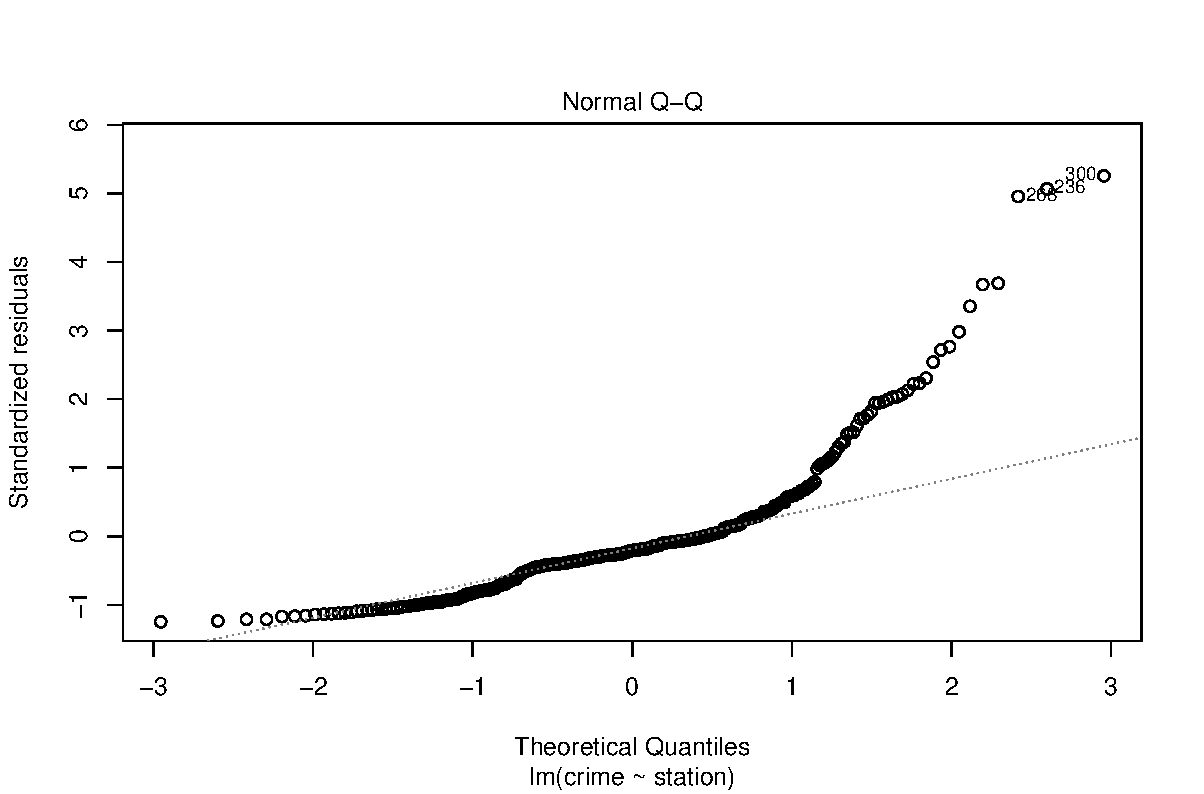
\includegraphics[scale=0.6]{figures/crime-qqplot.pdf}
    \caption{QQ-Norm Plot for Level-Dummy Specification}
    \label{fig:crime-qqplot}
\end{figure}

\begin{figure}
    \centering
    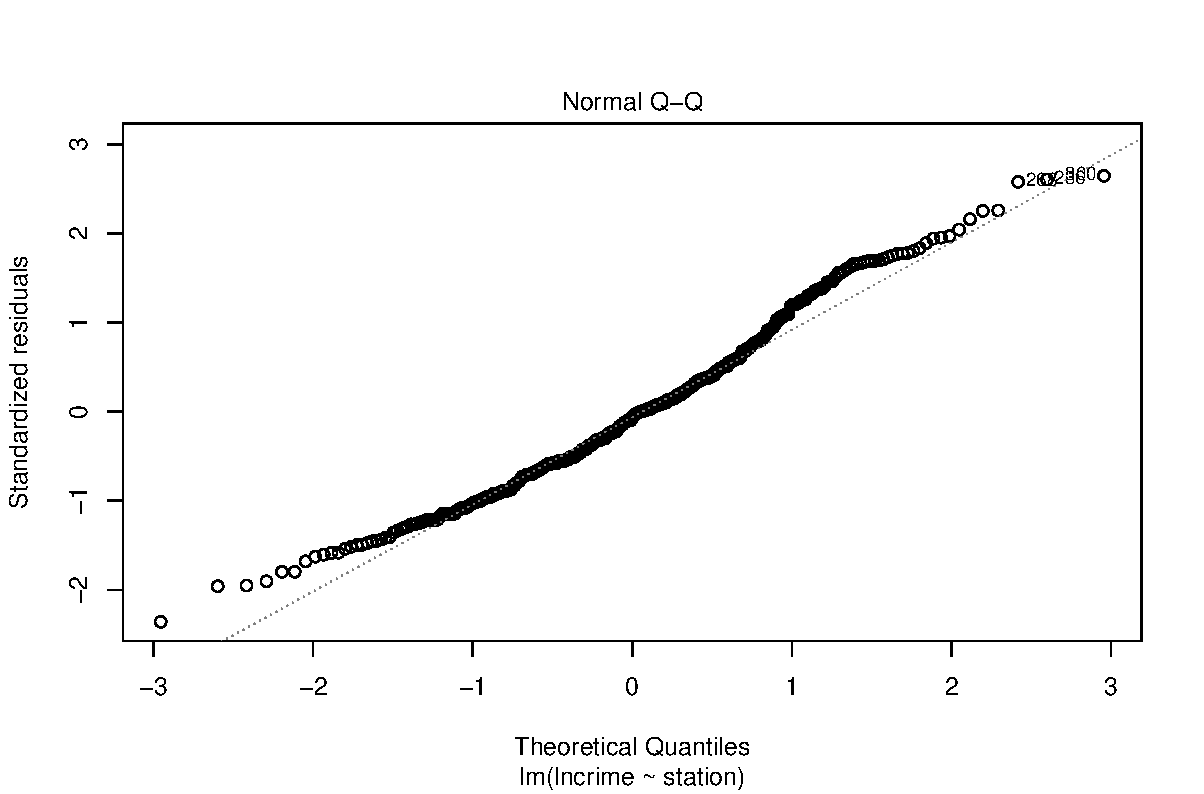
\includegraphics[scale=0.6]{figures/lncrime-qqplot.pdf}
    \caption{QQ-Norm Plot for Log-Dummy Specification}
    \label{fig:lncrime-qqplot}
\end{figure}



\end{document}
